\chapter{Introduction}
\label{chapterlabel1}

This thesis presents an in-depth technical explanation involved in building the proposed machine learning pipeline. While I tried to explain most techniques in detail intuitively without mathematical details, research or technical experience in the field of machine learning is required to fully understand it. If you find anything confusing, you can email me\footnote{\url{luoweilue@gmail.com}} to seek clarification.

\section{Background}

\subsection{2D Animation Pipeline}
2D animation is a manipulation of objects such that they appear as moving objects. It usually consists of a sequence of frames drawn by hand with computer-assisted technologies. The process of creating 2D animation consists of some labour-intensive tasks that depend on early-stage decisions. Once the development moves on to the next stage, it is very difficult or comes with a large cost to go back and change something that was not well thought out in the concept stage. This is known as the \textit{waterfall development model}\footnote{This is more of a term used in software development, but I think it is suitable to use here. See \url{https://en.wikipedia.org/wiki/Waterfall\_model} for more information.}. By improving this development process, we can save time and money, and have greater opportunities to improve the quality and quantity of work done, this could have a huge effect on the industry as a whole. In the following paragraphs, I will introduce (1) the current process for creating 2D animation;  (2) the proposed workflow; (3) the role of this master project and thesis. 


\subsubsection{Current Process}
In the current 2D animation creation process, the lead artist gives front-loaded creative input followed by labour-intensive tasks over which he has little control. I have listed the main stages of the existing 2D animation workflow as follows:

\begin{enumerate}
    \item \textbf{Key Poses / Layout} This is also called pose-to-pose (keyframe) drawing. It sets up major actions and placement in the scene.
    \item \textbf{Roughs / Inbetweening} This is the process for assigning timing and frame distribution. The lead animator will add timing notes for inbetweening artist in the form of frame charts that shows how the drawings should be distributed in time.
    \item \textbf{Cleanup / Inking} The rough pose-to-pose drawings are refined to inked clean drawings. This stage defines the styling and motion effects used from animation to animation. There are various line effects that can be used to exaggerate motions.
    \item \textbf{Coloring / Mattes} This is the final linework that adds colouring, shadows and highlights to the image.
\end{enumerate}

\begin{figure}
    \centering
    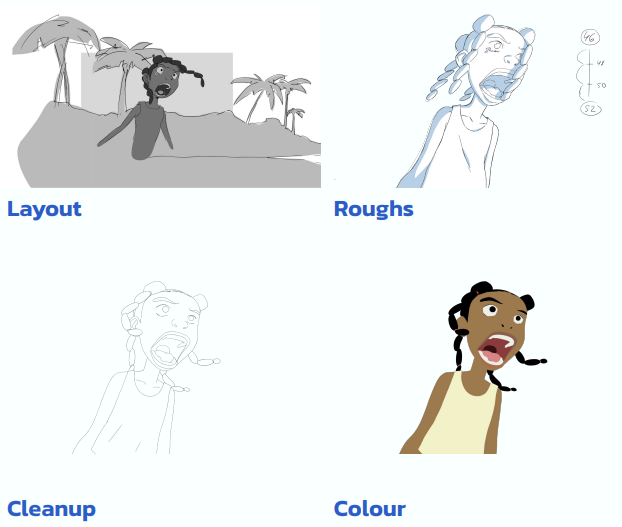
\includegraphics[width=0.75\textwidth]{images/introduction/stages.png}
    \caption[Sample frame for 4 stages of the workflow, including Layout, Roughs, Cleanup and Colour.]{Sample frame for 4 stages of the workflow, including Layout, Roughs, Cleanup and Colour.} 
    \label{fig:stages}
\end{figure}

We can see that the major actions and character placement are fixed after the first stage, there are only very rough sketches that define the starting and ending points of a transition (known as \textit{keyframes}), which is difficult to work with. We want the lead artist to get an accurate preview of what might be the final product and offers potential creative options. This is going to enhance and speed up the process of creating 2D animation.

\subsubsection{Proposed System}

\begin{figure}
    \centering
    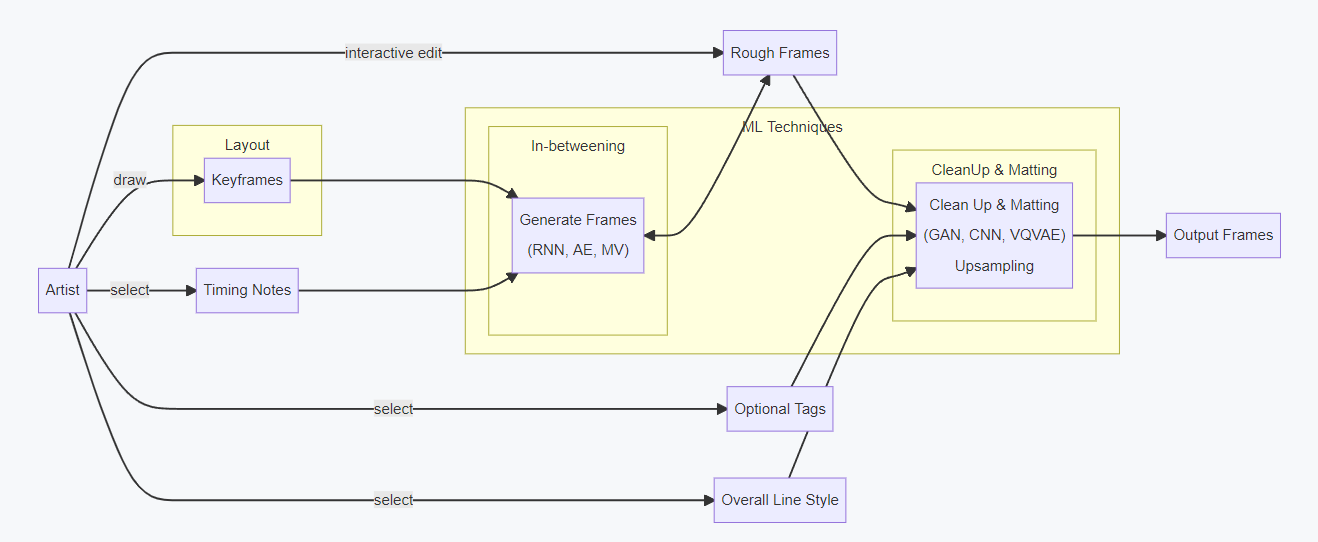
\includegraphics[width=1\textwidth]{images/introduction/proposed_workflow.png}
    \caption[Overview of proposed final workflow for the artist.]{Overview of proposed final workflow for the artist. The artist will produce a number of rough frames, with timing and style information. They will be fed into multiple machine learning (ML) pipelines to generate a preview of the final animation.} 
    \label{fig:proposed_worflow}
\end{figure}

In the proposed system, the artist will produce a number of rough keyframes with timing and style information. These frames will go through 4 ML pipelines, each consisting of a separate task: (1) cleaning up the rough sketches; (2) colouring; (3) frame interpolation (increase fps) and (4) upscaling (super-resolution).

The role of this master project is to (1) research each task, (2) develop a prototype model, (3) generate a proof-of-concept report and suggest future development direction. For this thesis, however, we will only discuss two areas that I have researched over the course of the master's project. This is to allow the thesis to be more focused and allows a more detailed explanation of each task. The two tasks I will be explaining in detail are (1) cleaning up the rough sketch and (2) colouring.


\section{General Approach}

\subsection{Image-to-Image Translation}
All four tasks fall into the field of Image-to-Image translation (I2I), which is a sub-field in Computer Vision. I2I refers to the task of transforming images from one domain to another so that they have the styles or characteristics from another domain. It has been gaining popularity in recent years due to its wide range of applications in computer vision problems such as image restoration, super-resolution, segmentation and pose-estimation. The scope of this project falls into two-domain, supervised I2I\cite{pangImagetoImageTranslationMethods2021}. Most recent research on I2I uses deep convolutional neural networks to learn a mapping function between and source and target domain. Pix2pix\cite{isolaImagetoImageTranslationConditional2018} first successfully apply deep convolutional conditional GAN to solve a wide range of I2I problems. However, Pix2pix itself suffers from a number of issues. For example, training might be unstable and error-prone as resolution increases\cite{wangHighResolutionImageSynthesis2018}; and unable to capture complex scene structure\cite{tangMultiChannelAttentionSelection2019}. Thus we will not directly apply it in our tasks, however, most models are either inspired by or follow the same architecture as Pix2pix.

\subsection{Pretraining}
Many researchers found that in computer vision tasks, it is generally useful to pre-train the model with a large amount of data and then finetune to downstream tasks\cite{baoBEiTBERTPreTraining2021, weiMaskedFeaturePrediction2021, newellHowUsefulSelfSupervised2020}. This is especially suitable in the context of this master project because the amount of data provided is a subset of all available data\cite{newellHowUsefulSelfSupervised2020}.

Pretraining can be seen as a form of weight initialization, and weight initialization is important when training neural networks. In the early days, some researchers initialize their neural network's weight to all zeros, and they soon find that this results in the \textit{symmetry problem} (see appendix \ref{app:ml:sym}), which makes the network harder to learn. Some researchers proposed random initialization, which works well in some cases. Still, if you are unlucky, you can run into initialization that is either too large or too small, which will result in exploding and vanishing gradient problems, respectively (see appendix \ref{app:ml:van_grad}). An popular alternative is Xavier initialization\cite{glorotUnderstandingDifficultyTraining2010} (see appendix \ref{app:ml:van_grad:weight_init}).


\begin{figure}
    \centering
    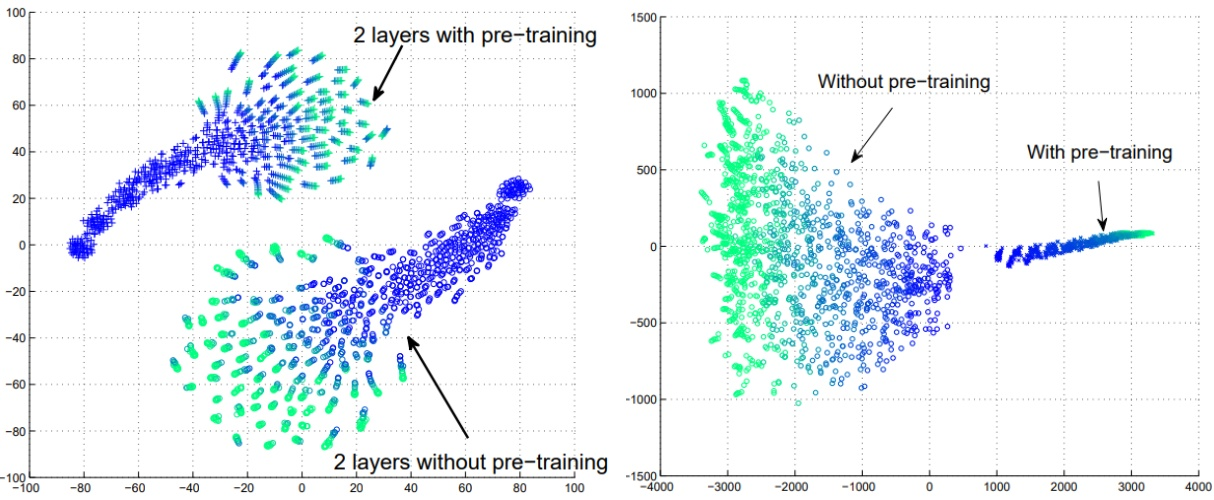
\includegraphics[width=1\textwidth]{images/introduction/pretrain_vis.jpg}
    \caption[Visualization of training progress of simple 2-layer networks.]{Visualization of training progress of simple 2-layer networks. Left is visualized with t-SNE (see appendix \ref{app:stat:tsne}) and right is visualized with ISOMAP (see appendix \ref{app:stat:isomap}) Color from blue to cyan indicates a progression in training iterations. Fifty of them are with pretraining (crosses), and another 50 are without pretraining (circles). We can observe that training with pretraining is generally faster and more stable than training without pretraining.\cite{erhanWhyDoesUnsupervised}} 
    \label{fig:pretrain_tsne}
\end{figure}

Although Xavier can improve initialization mathematically, the network will likely start far from the optimum. Pretraining on the other hand, when applied on a similar task, allow the model to start closer to the optimum, improving convergence time by reusing patterns learnt and improving model robustness\cite{hendrycksUsingPreTrainingCan2019} (see figure \ref{fig:pretrain_robustness}).


\begin{figure}
    \centering
    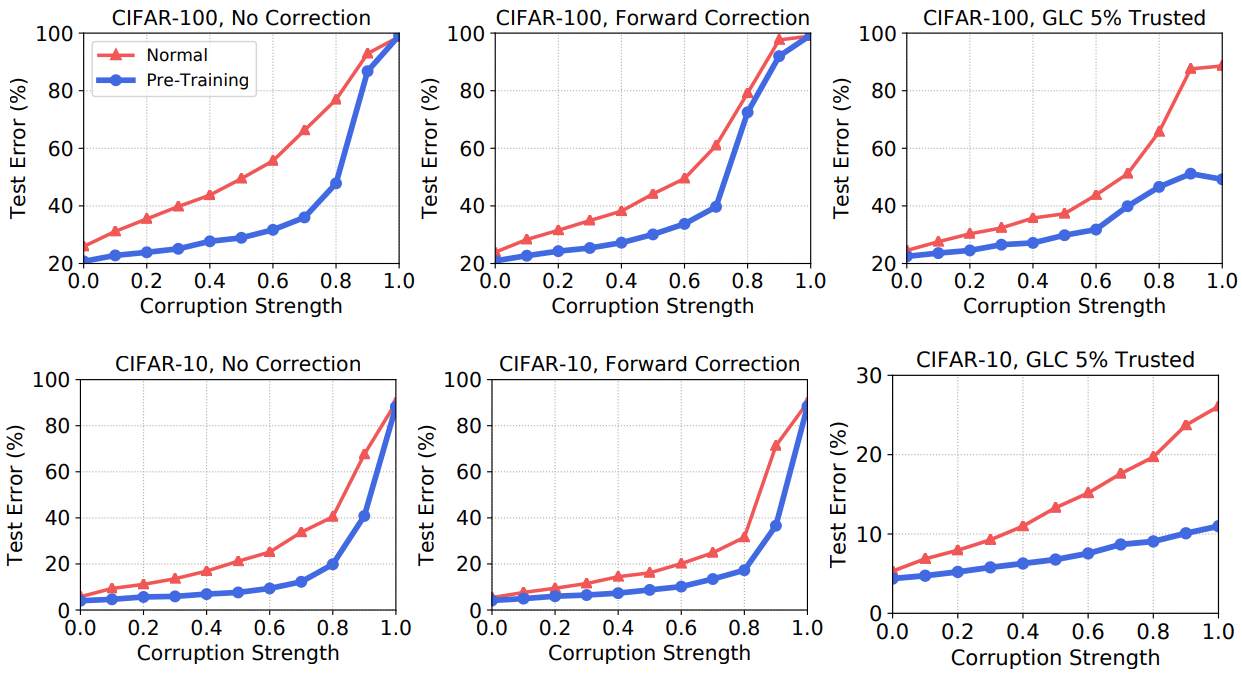
\includegraphics[width=0.75\textwidth]{images/introduction/pretrain_robustness.png}
    \caption[Classification error rate for a typical Wide ResNet\cite{zagoruykoWideResidualNetworks2017} on the CIFAR-10 and CIFAR-100 dataset with varying \textit{corruption strength} on the label during training.]{Classification error rate for a typical Wide ResNet\cite{zagoruykoWideResidualNetworks2017} on the CIFAR-10 and CIFAR-100 dataset with varying \textit{corruption strength} on the label during training. \textit{Corruption strength} refers to the probability that a training label is incorrect. We can observe that pretraining always outperforms training from scratch.} 
    \label{fig:pretrain_robustness}
\end{figure}

However, it is worth noting that pretraining does not necessarily improve result quality when a large training dataset is provided. Recent work showed that the benefits of pretraining diminish exponentially with increasing training data available. When sufficient data is provided, pretraining merely speeds up training on vision tasks\cite{heRethinkingImageNetPretraining2018}. Some studies even suggest that the pre-trained model performs worse because it is difficult for weights to abandon previously learned patterns, although it is theoretically possible\cite{el-noubyAreLargescaleDatasets2021}. 

Besides finetuning for downstream tasks, it can also be used as a feature extractor to enhance the network's capability for a variety of vision tasks. A popular choice is pre-trained vision transformer\cite{dosovitskiyImageWorth16x162021}, which is an attention-based network that achieved comparative results with SOTA convolutional neural network while requiring less computation. Some studies even directly used pre-trained feature extractors for vision classification tasks and achieved modest accuracy\cite{awaisCanPretrainedConvolutional2020}.


\subsection{Preprocessing}

\begin{figure}
    \centering
    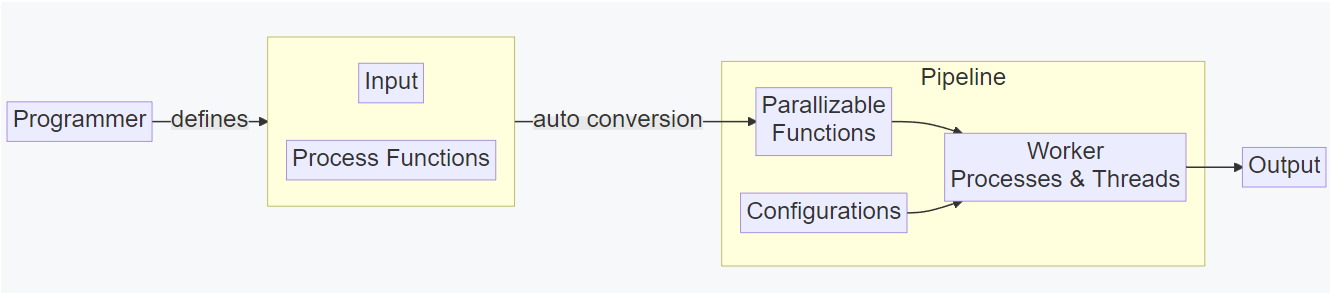
\includegraphics[width=1.0\textwidth]{images/introduction/preprocess_pipeline.png}
    \caption[Overview of Preprocessing pipeline.]{Overview of Preprocessing pipeline. In a typical use case, the programmer will first define a set of input and processing functions, feeds them into the pipeline and runs it. The pipeline will automatically convert the inputs into parallelizable functions and split them evenly across processes and threads for efficient processing, and finally, produce the processed output.} 
    \label{fig:preprocess_pipeline}
\end{figure}

There is a need for processing a large number of image files into a specific format, size and directory for this master project. To achieve this, I developed a small generalized multiprocessing \& multithreading pipeline in Python\cite{WelcomePythonOrg}. Together with pre-built modular processing functions, it provides a set of flexible and maintainable procedures for processing (see figure \ref{fig:preprocess_pipeline} for more details).

Regarding the NoGhost dataset, two major issues must be fixed before feeding into the machine learning pipelines to perform any data augmentation. 

The first issue is that there are many empty frames in the dataset, and for frames that are not empty, the character usually only occupies a small region of the image. If we feed images that are mostly empty into the machine learning models, it may just learn to produce empty output since it can match reasonably well with the target image distribution. The solution is to simply delete any empty frame and crop the empty region of the image. The algorithm is pretty straightforward, and it can be used to process efficiently. There are ~2000 images left after the cleaning.

The second issue is similar frames. Very often there are few differences between frames, and we have to remove them so that the resulting dataset is balanced. Otherwise, the models will bias toward characters that appear very often in the animation, leading to overfitting issues. To filter similar images efficiently, an image hashing algorithm is required. The idea is to represent images as a sequence of bytes such that similar images will get the same sequence. When given a new image, we only need to compute its hash and check whether we have seen it before. To accomplish this, we need an appropriate image hashing algorithm that is both efficient and collusion-resistant. Several well-known image hashing algorithms (see appendix \ref{app:misc:image_hashing}), and I chose the difference hashing algorithm as it balances speed and false positive well. There are ~500 images left after filtering.

In terms of generating training pairs, the current algorithm first matches the directory, sorts the images in the directory by filename and matches these images sequentially. The directory is matched by creating an identifier, this identifier is the result of removing numbers, and type-specific keywords, such as \textit{COL} and \textit{COLOUR} from the full directory name, and then directories with the same identifier are matched.

Some other preprocessing procedures exist, but they are mainly implementation details such as combining two images into one to reduce the chance of mixing and orders in the raw dataset are preserved to ensure reproducibility. Therefore I will not explain in detail here.

\subsection{Evaluation}
Note that in this thesis, we do not evaluate the output based on quantitative measures such as PSNR and SSIM. This is because this master project contributes to an industrial project, which has more implications than a research-focused project. For example, the stability and robustness of the model may be more important than a slight performance gain. In addition, most advancements in the network-generated anime-style image can be easily seen through plain eyes. Moreover, these measurements do not reflect other aspects of the image such as style variations which can have a large impact on the overall appearance of the anime-style image.

%Pretraining + finetuning + feature content loss + WGAN-GP, cGAN + U-Net

% Tobias says not relevant
% \subsection{Diffusion Model}
% Recently, diffusion model has been gaining popularity and shown comparative benchmarks on various computer vision tasks\cite{sahariaPaletteImagetoImageDiffusion2022, dhariwalDiffusionModelsBeat2021}. Although it is relatively new and has not been studied extensively and I did not apply them directly. I will briefly introduce them in case of interest in the future because it is highly potential.

% Diffusion model can be traced back to 2015 when researchers proposed a generative machine learning approach that is highly flexible and computationally tractable\cite{sohl-dicksteinDeepUnsupervisedLearning2015}. The idea is to develop a forward diffusion process that systematically and slowly erases the structure in the data, and then learn a backward diffusion process that recovers it. However, it did not attract much attention. Later, a stochastic differential equation that transforms complex data distribution to a known prior distribution based on the diffusion process was presented\cite{songScoreBasedGenerativeModeling2021}. It showed that the diffusion model can produce comparative performance in certain image generation tasks like inpainting by slowly introducing Gaussian noise into the forward diffusion process, and then learning its reverse process. A denoising diffusion model\cite{hoDenoisingDiffusionProbabilistic2020} also showed that it is capable of generating high-quality images.

% \todo[inline]{TODO: introduce diffusion model researches}

% \section{Evaluation Methods}
%mostly by eye, we can compute the PSNR and SSIM, but, generally, the eye is enough.
%Some stuff about things.\cite{example-citation} Some more things. 

%Inline citation: \bibentry{example-citation}

% This just dumps some pseudo-Latin in so you can see some text in place.
%\blindtext
